\documentclass{article}
\usepackage{amsfonts}
\usepackage{amsmath}
\usepackage{indentfirst}
\usepackage{graphicx} % Required for inserting images

\title{Modeling Infant Birthweight Distribution Using Kernel Density Estimation}
\author{Austin Paczkowski}
\date{\today}

\begin{document}

\maketitle

\section{Introduction}

In any experiment with collected data, the context, properties, and assumptions behind said data are the engine that powers hypothesis testing. Naturally, a scientist may wonder about the distribution of their collected data. While there are a multitude of methods that can be applied to visualize data such as histograms, scatter plots, and box plots, these methods are rather naive as none of them are sufficient for predicting the likelihood of future observations. As such, Kernel Density Estimation (KDE), a widely used non-parametric statistical method, serves to do just that by transforming a collection of discrete observations into an estimated probability distribution function of the data. Using the estimated pdf from KDE, we can visualize data and assign likelihoods of future theoretical values based on known observations. 

In this paper, we will work on the \textit{birthwt} data from the MASS library \cite{masS}, containing 189 infant weight measurements, low-weight classifications, and risk factors of infant mothers. With this data, we will apply KDE in R, use additional statistical, data-wrangling, and data-analysis techniques detailed later, and finish by modeling distributions derived from conclusions about the data.

\section{Mathematical Theory}

\subsection{Explaining KDE Mathematically}

Before applying KDE and analyzing the introduced data, we need to establish its mathematical definition and derive some useful properties. As such, the KDE estimates the probability distribution function $\hat f(x)$ for 1 dimension:

\begin{equation}
    \hat f_h(x) = \frac{1}{n}\sum_{i=1}^n K_h(x - x_i)
\end{equation}

where

\begin{equation}
    K_h(x) = \frac{1}{h}K(x)
\end{equation}

\newpage

In English, KDE estimates the pdf of discrete data by assigning a choice of kernel $K(x_i)$ using the bandwidth parameter $h$ on the range $h = \sigma$ for the Gaussian kernel, and $\mathbf{1}_{[x-\frac{h}{2}, x+\frac{h}{2}]}$ for non-Gaussian kernels, and combining each of these kernels to estimate the distribution. In other words, one can think of the estimate as a distribution composed of a sum of distributions. In theory, one could use any kernel for the parameter $K$. However, some distributions such as $Beta(\alpha \ne \beta)$ and $Gamma(\alpha \ne \infty)$ are skewed, providing presumptions about the data that may be false. As such, one should typically use centered distributions such as Gaussian, Uniform, and Epanechnikov 
as the kernel for K as these are not skewed.

\subsection{Bandwidth Choice}

While choosing a kernel is relatively trivial, deciding an appropriate bandwidth to represent is not as simple. If we choose a relatively small bandwidth value, our estimation will not be smooth and is considered underfitted, as seen in the left figure below. On the contrary, choosing a relatively large bandwidth value will give an overfitted estimation that loses unique features in our distribution, as seen in the middle figure below. As such, we want to find a bandwidth that is properly fitted: one that pronounces the unique properties in our distribution while appearing visually smooth as seen on the right below.

\begin{figure}[h]
    \centering
    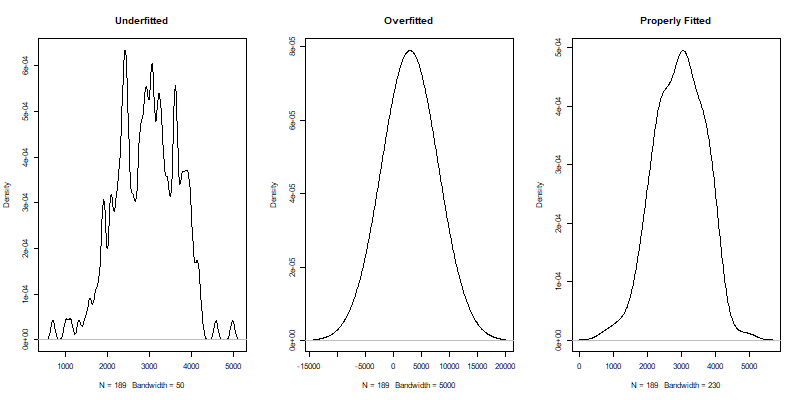
\includegraphics[scale = 0.33]{volume/KDE_FitComparison.png}
    \caption{Bandwidth Fit Classifications}
    \label{fig:fit-classification}
\end{figure}

With this in mind, there are three limits in Equation (1) worth considering: when $n \rightarrow \infty$, when $h \rightarrow 0$, and when $h \rightarrow \infty$. When the number of observations becomes sufficiently large, their distribution will approach a normal distribution by the Central Limit Theorem as long as the measurements are independently and identically distributed.

\begin{figure}[h]
    \centering
    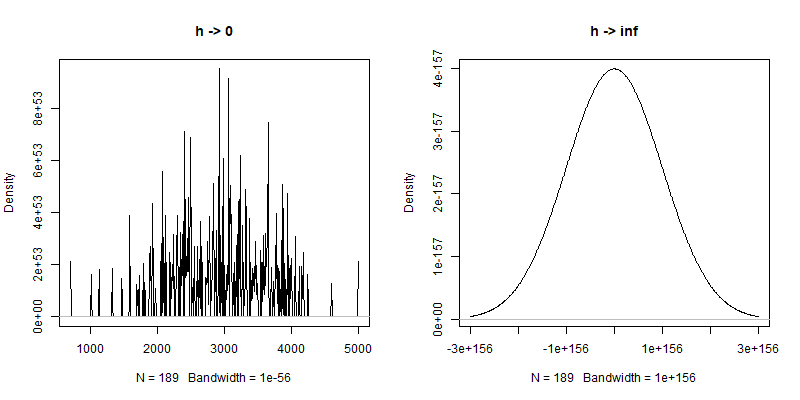
\includegraphics[scale = 0.33]{volume/BandwidthLimits.png}
    \caption{Visualizing Bandwidth Limits}
    \label{fig:band-limts}
\end{figure}

\newpage

When h approaches 0, the distribution becomes a sum of Dirac delta functions with infinite probability at $x_i$ in the left figure above (2), namely:

\begin{equation}
    lim_{h \rightarrow0 } \hat f_h(x) = \sum_{i=1}^n \delta(x_i)
\end{equation}

When h approaches $\infty$, the distribution of data approaches the kernel with $h = \sigma$ for the Gaussian kernel and $\mathbf{1}_{[x-\frac{h}{2}, x+\frac{h}{2}]}$ for non-Gaussian kernels in the right figure above (2), namely:

\begin{equation}
    lim_{h \rightarrow \infty }\hat f_h(x)  \xrightarrow{D}K
\end{equation}

\subsection{Bandwidth Estimation}

After examining bandwidth limits to conceptualize bandwidth context, we still need a protocol for choosing a bandwidth. Fortunately, this is an optimization problem where we minimize the Mean Integrated Standard Error below (5) of h by solving for its derivative equal to 0.

\begin{equation}
    MISE(h) = E[\int_x (\hat f_h(x) - f(x))^2 dx]
\end{equation}

However, MISE contains the true density of our data $f(x)$ as one of the terms, meaning we cannot find the true optimal bandwidth. As such, we need to apply some method that chooses an estimate $\hat h$ for the bandwidth. As such, we will briefly examine four different algorithms that we will use later in our analysis: Silverman's Rule of Thumb, Scott's Rule of Thumb, Plug-In Selectors, and Leave One Out Cross-Validation (LOOCV) \cite{refId0}.

\newpage

First, Silverman and Scott's Rule of Thumb are simple estimators for h that leverage the estimated standard deviation of the data using equations (6) and (7) below.

\begin{equation}
    \hat h_{Silverman} \approx 1.059 \hat \sigma n^{-\frac{1}{5}}
\end{equation}

\begin{equation}
    \hat h_{Scott} \approx 0.9min(\hat \sigma, \frac{IQR}{1.34})n^{-\frac{1}{5}}
\end{equation}

Silverman's Rule of Thumb minimizes the MISE \cite{refId0} while Scott's Rule of Thumb adds extra flexibility to deal with potentially skewed data by leveraging the Interquartile Range. Next, the Plugin Selector Method leverages properties of the inputted data to get an estimate of h and then uses that estimate to derive more properties about the data. This method iterates until the bandwidth deviates by less than a given epsilon between steps if it converges. Finally, Leave One Out Cross-Validation (LOOCV) estimates a bandwidth by performing CV-tests n times, summing up the errors, and choosing a bandwidth that minimizes the error in the LOOCV. With this mathematical theory examined, we now have the background, tools, and awareness of relevant statistical methods to aid us in performing meaningful data analysis on the \textit{birthwt} data introduced earlier.

\section{Using KDE for Data Analysis}

\subsection{Analysis Preparation}

First, we recall the dataset \textit{birthwt} in full detail below (3):

\begin{figure}[h]
    \centering
    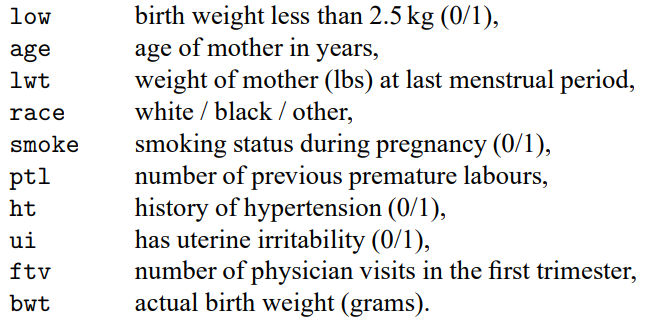
\includegraphics[scale = 1]{volume/birthwt_properties.PNG}
    \caption{birthwt Dataframe Variables}
    \label{fig:birthwt-table}
\end{figure}

\newpage

In preparing the data, we change each categorical variable to factors, dropping \texttt{low} as it has strong colinearity with \texttt{birthwt} as our response of interest. While we can perform high-level analysis, we want to keep this one-dimensional to remain in the scope of this paper. As such, we will perform a simple linear regression of these factors, find a single factor variable of interest, and apply KDE between the levels of said factor to visualize the difference in birth weight. Performing linear regression and calling \texttt{summary} gives our coefficients and ANOVA tests below (4):

\begin{figure}[h]
    \centering
    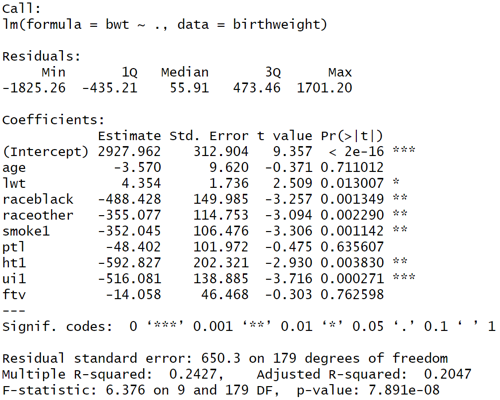
\includegraphics[scale = 1]{volume/summaryLinReg.PNG}
    \caption{Linear Regression on cleaned birthwt}
    \label{fig:lin-reg}
\end{figure}

From the regression model, \texttt{ui1} (Uterine Irritability present in the infant's mother) is the most significant factor towards smaller infant weights, with an ANOVA F-test p-value less than 0.0003. As such, we will apply KDE to visualize the distribution of infant weights in \texttt{ui0} vs. \texttt{ui1}.

\subsection{Choosing our Kernel}

With \texttt{ui} already classified as a factor in our R data frame, we will apply KDE with different Kernels, keep the bandwidth selection the same in each, and choose an appropriate kernel. As such, we will use Scott's Rule of Thumb bandwidth estimation in each density plot, having \texttt{ui0} and \texttt{ui1} as the row plots, and the Gaussian, Uniform, and Epanechnikov kernel in the column plots below (5).

\newpage

\begin{figure}[h]
    \centering
    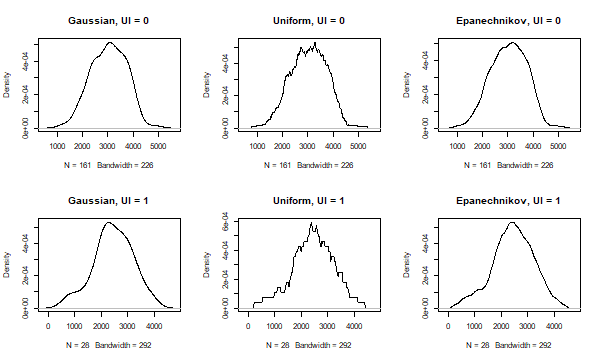
\includegraphics[scale = 0.4]{volume/KDE_kernel_choices.png}
    \caption{Kernel Choice Plot Matrix}
    \label{fig:kernel-choices}
\end{figure}

Visually, the Uniform kernel appears underfitted, especially in the \texttt{ui1} plot with only $N_1 = 28$ observations. On the contrary, the Gaussian and Epanechnikov kernels are properly fitted, making both kernels viable choices. For our analysis, we will choose the Epanechnikov kernel as it minimizes the Mean Squared Error (MSE) of our data \cite{refId0} while keeping key traits of our data's distribution.

\subsection{Choosing our Bandwidth}

With our kernel choice established, we will choose a bandwidth $\hat h$ from one of the four methods introduced earlier. Using the Epanechnikov kernel in each density plot, having \texttt{ui0} and \texttt{ui1} as the row plots, and Scott's RoT, Silverman's RoT, biased Cross-Validation (reduces variance), and Plug-in Selection in the column plots, we get the resulting plot matrix below (6).

\begin{figure}[h]
    \centering
    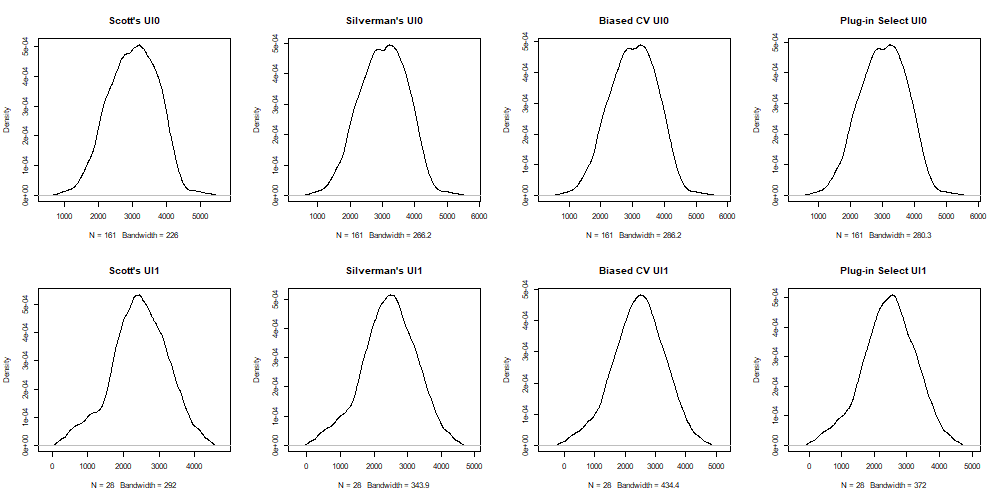
\includegraphics[scale = 0.25]{volume/KDE_bandwidth_choices.png}
    \caption{Bandwidth Method Choice Plot Matrix}
    \label{fig:bw-plots}
\end{figure}

\newpage

All four bandwidth selection techniques give distributions that are properly fitted, making any of them a viable choice. As such, we will choose Scott's Rule of Thumb to model our distribution due to its simplicity and lower runtime \cite{Raykar01012010}.

\subsection{Putting it All Together}

After separating our data by Uterine Irritability classification, settling on an Epanechnikov Kernel, and applying Scott's Rule of thumb bandwidth estimation, we will model the probability density estimates for \texttt{ui0} in red, \texttt{ui1} in blue, and the total distribution in black below (7).

\begin{figure}[h]
    \centering
    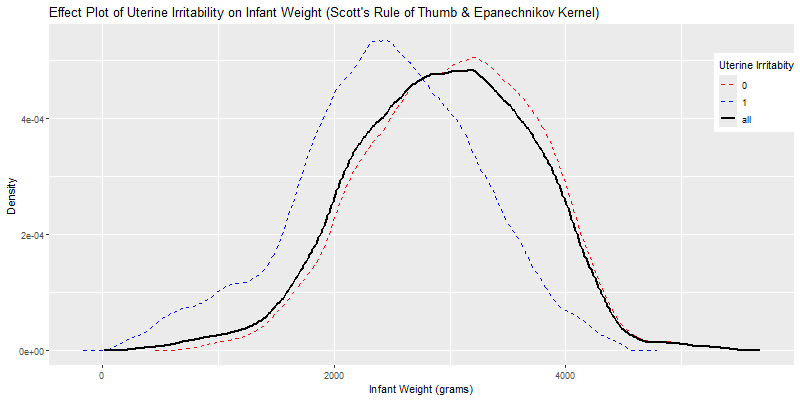
\includegraphics[scale = 0.4]{volume/KDE_UIPlot.png}
    \caption{Effect Plot of Uterine Irritability using Kernel Density Estimation}
    \label{fig:effect-plot-KDE}
\end{figure}

From this visualization, the distribution of infant weight is more appropriately modeled as a Gaussian mixture, separated by uterine irritability classification in mothers compared to a singular, homogeneous distribution.

%%

\section{Conclusion and Further Analysis Discussion}

In this paper, we introduced Kernel Density Estimation, contextualized the mathematical theory and background behind KDE, applied multiple KDE's bandwidth and kernel selection techniques, and visualized infant weight distributions between the different levels of \texttt{ui} on the real-world dataset \textit{birthwt}, signifying uterine irritability in mothers as a key risk factor for low-weight infants. With this paper's analysis concluded, there are a plethora of directions one may take in deeper analysis of this data. For one, our uterine irritability analysis suggests implementing $\hat f_{h, UI}(x)$ as a Gaussian Mixture Kernel Density Estimation \cite{gmmKDE} if one wants to conduct a more advanced analysis or model. Second, one could perform Multidimensional KDE \cite{masS}, usually on $d = 2$ variables as a 3D graph, to model additional attributes and visualize the correlation between variables in the data. Finally, and most significantly, one may want to add weights to classifications as $N_0 >> N_1$ where only $N_1 = 28$ \texttt{ui1} observations were present compared to $N_0 = 161$ \texttt{ui0} observations. As such, the total Kernel Density Estimate was heavily biased towards the \texttt{ui0} distribution. This is why a Gaussian Mixture model was suggested by our KDE visualization, as we did not add weights to the classifications. Ultimately, these are only a handful of suggestions that are meant to demonstrate how flexible and configurable the non-parametric statistical method KDE is for data analysis.

%References%

\bibliographystyle{plain}
\bibliography{references}

\end{document}